\documentclass[12pt]{extreport}
\usepackage[T2A]{fontenc}
\usepackage[utf8]{inputenc}        % Кодировка входного документа;
                                    % при необходимости, вместо cp1251
                                    % можно указать cp866 (Alt-кодировка
                                    % DOS) или koi8-r.

\usepackage[english,russian]{babel} % Включение русификации, русских и
                                    % английских стилей и переносов
%%\usepackage{a4}
%%\usepackage{moreverb}
\usepackage{amsmath,amsfonts,amsthm,amssymb,amsbsy,amstext,amscd,amsxtra,multicol}
\usepackage{indentfirst}
\usepackage{verbatim}
\usepackage{tikz} %Рисование автоматов
\usetikzlibrary{automata,positioning}
%\usepackage{multicol} %Несколько колонок
\usepackage{graphicx}
\usepackage[colorlinks,urlcolor=blue]{hyperref}
\usepackage[stable]{footmisc}

%% \voffset-5mm
%% \def\baselinestretch{1.44}
\renewcommand{\theequation}{\arabic{equation}}
\def\hm#1{#1\nobreak\discretionary{}{\hbox{$#1$}}{}}
\newtheorem{Lemma}{Лемма}
\theoremstyle{definiton}
\newtheorem{Remark}{Замечание}
%%\newtheorem{Def}{Определение}
\newtheorem{Claim}{Утверждение}
\newtheorem{Cor}{Следствие}
\newtheorem{Theorem}{Теорема}
\theoremstyle{definition}
\newtheorem{Example}{Пример}
\newtheorem*{known}{Теорема}
\def\proofname{Доказательство}
\theoremstyle{definition}
\newtheorem{Def}{Определение}

%% \newenvironment{Example} % имя окружения
%% {\par\noindent{\bf Пример.}} % команды для \begin
%% {\hfill$\scriptstyle\qed$} % команды для \end






%\date{22 июня 2011 г.}
\let\leq\leqslant
\let\geq\geqslant
\def\MT{\mathrm{MT}}
%Обозначения ``ажуром''
\def\BB{\mathbb B}
\def\CC{\mathbb C}
\def\RR{\mathbb R}
\def\SS{\mathbb S}
\def\ZZ{\mathbb Z}
\def\NN{\mathbb N}
\def\FF{\mathbb F}
%греческие буквы
\let\epsilon\varepsilon
\let\es\varnothing
\let\eps\varepsilon
\let\al\alpha
\let\sg\sigma
\let\ga\gamma
\let\ph\varphi
\let\om\omega
\let\ld\lambda
\let\Ld\Lambda
\let\vk\varkappa
\let\Om\Omega
\def\abstractname{}

\def\R{{\cal R}}
\def\A{{\cal A}}
\def\B{{\cal B}}
\def\C{{\cal C}}
\def\D{{\cal D}}

%классы сложности
\def\REG{{\mathsf{REG}}}
\def\CFL{{\mathsf{CFL}}}


%%%%%%%%%%%%%%%%%%%%%%%%%%%%%%% Problems macros  %%%%%%%%%%%%%%%%%%%%%%%%%%%%%%%


%%%%%%%%%%%%%%%%%%%%%%%% Enumerations %%%%%%%%%%%%%%%%%%%%%%%%

\newcommand{\Rnum}[1]{\expandafter{\romannumeral #1\relax}}
\newcommand{\RNum}[1]{\uppercase\expandafter{\romannumeral #1\relax}}

%%%%%%%%%%%%%%%%%%%%% EOF Enumerations %%%%%%%%%%%%%%%%%%%%%

\usepackage{xparse}
\usepackage{ifthen}
\usepackage{bm} %%% bf in math mode
\usepackage{color}
%\usepackage[usenames,dvipsnames]{xcolor}

\definecolor{Gray555}{HTML}{555555}
\definecolor{Gray444}{HTML}{444444}
\definecolor{Gray333}{HTML}{333333}


\newcounter{problem}
\newcounter{uproblem}
\newcounter{subproblem}
\newcounter{prvar}

\def\beforPRskip{
	\bigskip
	%\vspace*{2ex}
}

\def\PRSUBskip{
	\medskip
}


\def\pr{\beforPRskip\noindent\stepcounter{problem}{\bf \theproblem .\;}\setcounter{subproblem}{0}}
\def\pru{\beforPRskip\noindent\stepcounter{problem}{\bf $\mathbf{\theproblem}^\circ$\!\!.\;}\setcounter{subproblem}{0}}
\def\prstar{\beforPRskip\noindent\stepcounter{problem}{\bf $\mathbf{\theproblem}^*$\negthickspace.}\setcounter{subproblem}{0}\;}
\def\prpfrom[#1]{\beforPRskip\noindent\stepcounter{problem}{\bf Задача \theproblem~(№#1 из задания).  }\setcounter{subproblem}{0} }
\def\prp{\beforPRskip\noindent\stepcounter{problem}{\bf Задача \theproblem .  }\setcounter{subproblem}{0} }

\def\prpvar{\beforPRskip\noindent\stepcounter{problem}\setcounter{prvar}{1}{\bf Задача \theproblem \;$\langle${\rm\Rnum{\theprvar}}$\rangle$.}\setcounter{subproblem}{0}\;}
\def\prpv{\beforPRskip\noindent\stepcounter{prvar}{\bf Задача \theproblem \,$\bm\langle$\bracketspace{{\rm\Rnum{\theprvar}}}$\bm\rangle$.  }\setcounter{subproblem}{0} }
\def\prv{\beforPRskip\noindent\stepcounter{prvar}{\bf \theproblem\,$\bm\langle$\bracketspace{{\rm\Rnum{\theprvar}}}$\bm\rangle$}.\setcounter{subproblem}{0} }

\def\prpstar{\beforPRskip\noindent\stepcounter{problem}{\bf Задача $\bf\theproblem^*$\negthickspace.  }\setcounter{subproblem}{0} }
\def\prdag{\beforPRskip\noindent\stepcounter{problem}{\bf Задача $\theproblem^{^\dagger}$\negthickspace\,.  }\setcounter{subproblem}{0} }
\def\upr{\beforPRskip\noindent\stepcounter{uproblem}{\bf Упражнение \theuproblem .  }\setcounter{subproblem}{0} }
%\def\prp{\vspace{5pt}\stepcounter{problem}{\bf Задача \theproblem .  } }
%\def\prs{\vspace{5pt}\stepcounter{problem}{\bf \theproblem .*   }
\def\prsub{\PRSUBskip\noindent\stepcounter{subproblem}{\sf \thesubproblem .} }
\def\prsubr{\PRSUBskip\noindent\stepcounter{subproblem}{\bf \asbuk{subproblem})}\;}
\def\prsubstar{\PRSUBskip\noindent\stepcounter{subproblem}{\rm $\thesubproblem^*$\negthickspace.  } }
\def\prsubrstar{\PRSUBskip\noindent\stepcounter{subproblem}{$\text{\bf \asbuk{subproblem}}^*\mathbf{)}$}\;}

\newcommand{\bracketspace}[1]{\phantom{(}\!\!{#1}\!\!\phantom{)}}

\DeclareDocumentCommand{\Prpvar}{ O{null} O{} }{
	\beforPRskip\noindent\stepcounter{problem}\setcounter{prvar}{1}{\bf Задача \theproblem
% 	\ifthenelse{\equal{#1}{null}}{  }{ {\sf $\bm\langle$\bracketspace{#1}$\bm\rangle$}}
%	~\!\!(\bracketspace{{\rm\Rnum{\theprvar}}}).  }\setcounter{subproblem}{0}
%	\;(\bracketspace{{\rm\Rnum{\theprvar}}})}\setcounter{subproblem}{0}
%
	\,{\sf $\bm\langle$\bracketspace{{\rm\Rnum{\theprvar}}}$\bm\rangle$}
	~\!\!\! \ifthenelse{\equal{#1}{null}}{\!}{{\sf(\bracketspace{#1})}}}.

}
%\DeclareDocumentCommand{\Prpvar}{ O{level} O{meta} m }{\prpvar}


\DeclareDocumentCommand{\Prp}{ O{null} O{null} }{\setcounter{subproblem}{0}
	\beforPRskip\noindent\stepcounter{problem}\setcounter{prvar}{0}{\bf Задача \theproblem
	~\!\!\! \ifthenelse{\equal{#1}{null}}{\!}{{\sf(\bracketspace{#1})}}
	 \ifthenelse{\equal{#2}{null}}{\!\!}{{\sf [\color{Gray444}\,\bracketspace{{\fontfamily{afd}\selectfont#2}}\,]}}}.}

\DeclareDocumentCommand{\Pr}{ O{null} O{null} }{\setcounter{subproblem}{0}
	\beforPRskip\noindent\stepcounter{problem}\setcounter{prvar}{0}{\bf\theproblem
	~\!\!\! \ifthenelse{\equal{#1}{null}}{\!\!}{{\sf(\bracketspace{#1})}}
	 \ifthenelse{\equal{#2}{null}}{\!\!}{{\sf [\color{Gray444}\,\bracketspace{{\fontfamily{afd}\selectfont#2}}\,]}}}.}

%\DeclareDocumentCommand{\Prp}{ O{level} O{meta} }

\DeclareDocumentCommand{\Prps}{ O{null} O{null} }{\setcounter{subproblem}{0}
	\beforPRskip\noindent\stepcounter{problem}\setcounter{prvar}{0}{\bf Задача $\bm\theproblem^* $
	~\!\!\! \ifthenelse{\equal{#1}{null}}{\!}{{\sf(\bracketspace{#1})}}
	 \ifthenelse{\equal{#2}{null}}{\!\!}{{\sf [\color{Gray444}\,\bracketspace{{\fontfamily{afd}\selectfont#2}}\,]}}}.
}

\DeclareDocumentCommand{\Prpd}{ O{null} O{null} }{\setcounter{subproblem}{0}
	\beforPRskip\noindent\stepcounter{problem}\setcounter{prvar}{0}{\bf Задача $\bm\theproblem^\dagger$
	~\!\!\! \ifthenelse{\equal{#1}{null}}{\!}{{\sf(\bracketspace{#1})}}
	 \ifthenelse{\equal{#2}{null}}{\!\!}{{\sf [\color{Gray444}\,\bracketspace{{\fontfamily{afd}\selectfont#2}}\,]}}}.
}


\def\prend{
	\bigskip
%	\bigskip
}




%%%%%%%%%%%%%%%%%%%%%%%%%%%%%%% EOF Problems macros  %%%%%%%%%%%%%%%%%%%%%%%%%%%%%%%



%\usepackage{erewhon}
%\usepackage{heuristica}
%\usepackage{gentium}

\usepackage[portrait, top=3cm, bottom=1.5cm, left=3cm, right=2cm]{geometry}

\usepackage{fancyhdr}
\pagestyle{fancy}
\renewcommand{\headrulewidth}{0pt}
\lhead{\fontfamily{fca}\selectfont {ФПМИ, Основные алгоритмы 2022} }
%\lhead{ \bf  {ТРЯП. } Семинар 1 }
%\chead{\fontfamily{fca}\selectfont {Вариант 1}}
\rhead{\fontfamily{fca}\selectfont Павлов М.А. Домашнее задание 11}
%\rhead{\small 04.2022}
\cfoot{}

\usepackage{titlesec}
\titleformat{\section}[block]{\Large\bfseries\filcenter {\setcounter{problem}{0}}  }{}{1em}{}


%%%%%%%%%%%%%%%%%%%%%%%%%%%%%%%%%%%%%%%%%%%%%%%%%%%% Обозначения и операции %%%%%%%%%%%%%%%%%%%%%%%%%%%%%%%%%%%%%%%%%%%%%%%%%%%% 
                                                                    
\newcommand{\divisible}{\mathop{\raisebox{-2pt}{\vdots}}}           
\let\Om\Omega


%%%%%%%%%%%%%%%%%%%%%%%%%%%%%%%%%%%%%%%% Shen Macroses %%%%%%%%%%%%%%%%%%%%%%%%%%%%%%%%%%%%%%%%
\newcommand{\w}[1]{{\hbox{\texttt{#1}}}}


\begin{document}
	

\pr Дан неориентированный граф $G = (V,E)$, веса рёбер которого не обязательно различны...

\prsubr Если к каждому ребру графа прибавить вес $w$, то каждое минимальное остовное дерево $G$ перейдёт в минимальное остовное дерево модифицированного графа.

	Да, это верное утверждение. (Вроде как даже рассматривали подобный случай на семинаре, но все равно распишу доказательство).

	Вспомним алгоритм Крускала построения минимального остовного дерева, который разбирался на семинаре: сначала мы сортируем ребра.
	Очевидно, что при добавлении к каждому ребру значение $w$ порядок ребер после сортировки не изменится.
	Значит, алгоритм в результате выдаст такое же минимальное остовное дерево, но его вес будет больше на $(n-1) \cdot w$, где $n$ -- количество вершин в графе.

\prsubr Если самое лёгкое ребро графа $G$ уникально, то оно входит в любое минимальное остовное дерево.

	Да, это верное утверждение.

	Вновь вспомним алгоритм Крускала. После сортировки ребер по весу самое легкое ребро будет самым легким (вот это поворот), следовательно, с него мы и начнем построение остова.
	Раз уж с него мы начинаем построение остова, то оно в любом случае будет принадлежать этому остову, то есть какой бы минимальный остов мы ни взяли, первое ребро гарантированно будет лежать в нем.

\prsubr Если ребро $e$ входит в некоторое минимальное остовное дерево, то оно является самым лёгким ребром из пересекающих некоторый разрез.

	Да, это верное утверждение. Докажем это сильное утверждение от противного.

	Предположим, что для каждого из разрезов, которые пересекает ребро $e$, можно найти более легкое ребро из этого разреза.
	Но в таком случае при любом разрезе графа выгоднее вместо ребра $e$ взять то самое более легкое ребро, откуда следует, что $e$ не будет лежать в остове, что противоречит условию.
	Значит, предположение неверно, а утверждение верно.

\prsubr Кратчайший путь между двумя вершинами является частью некоторого минимального остовного дерева.

	Это неправда. Контрпример мы рассматривали на семинаре, но я буду оригинальным и придумаю свой.

\begin{wrapfigure}
	\centering
	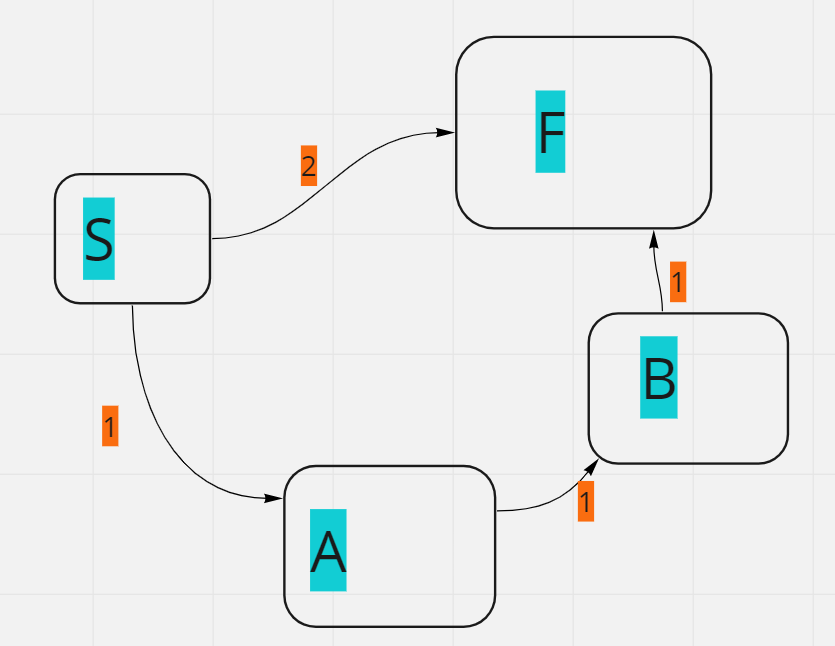
\includegraphics[scale=0.6]{graph}
	\caption{Контрпример}
\end{wrapfigure}

	Здесь множество минимальных остовных состоит из ребер $\{sa, ab, bf\}]$. Однако, кратчайший путь от $S$ до $F$ состоит из множества ребер $\{sf\}$, некоторые ребра которого не присутствуют ни в одном минимальном остовном дереве. Ура. Мы все доказали.

\medskip
\noindent{\textbf{Опредедение.}} Граф, который получается из графа $G$ удалением некоторых вершин и рёбер, называют \emph{(рёберным) подграфом} графа~$G$. В случае, если при изготовлении подграфа, рёбра удалялись только вместе с удалением вершин, подграф называют \emph{индуцированным}.
\medskip

\pr Пусть $T$ "--- минимальное остовное дерево графа $G$, а $H$ \ldots

	Предположим, что найдется ребро $(u, v)$, которое входит в $T$ и $H$, но не входит ни в какое минимальное остновное дерево $H$.
	Это значит, что существует ребро, соединяющее разрез $(A, B) : u \in A, v \in B$, такое, что его вес меньше веса $(u, v)$.
	Но в таком случае в графе $G$ появляется цикл, проходящий по этим двум ребрам. Очевидно, что для построения минимального остова нам необходимо
	будет взять все ребра, кроме самого тяжелого.

	Если из указанных выше ребер $(u, v)$ -- самое тяжелое, то убираем его. Но оно лежало в остове по предположение, значит, предположение неверно и первый случай доказан.

	Если оно не самое тяжелое, то найдется ребро, лежащее в этом цикле, которое тяжелее него. Но в таком случае мы не можем убрать его при построении минимального остова $H$, т.к. во всех циклах найдется ребро, тяжелее $(u, v)$.

	Получается, что $(u, v)$ в таком случае входит в минимальное остовное дерево графа $H$, что тоже противоречит предположению.

	Оба случая пришли к противоречию, значит, утверждение доказано.

\pr Рассмотрим алгоритм Union-Find без улучшения со сжатием путей\footnote{При вызове $\mathrm{Find}(x)$ все предки $x$ вместе с $x$ становятся детьми корня.}. Приведите последовательность из $m$ операций Union и Find над множеством из $n$ элементов, которая потребует времени $\Omega(m\log n)$.

	Предположим, что число вершин -- степень двойки. Тогда при построении на множестве вершин бинарного дерева мы можем рекурсивно объединять семьи на каждом уровне по парам.

	Далее запускаем Find для каждой вершины.

	Количество поисков совпадает с поделенным на 2 количеством вершин и равно $\frac{n}{2} = m$. Количество объединений равно $m$.
	Каждый поиск работает за $log n$.

	В результате у нас получается оценка $\theta(T) = \theta(mlogn) \Rightarrow \Omega(T) = \Omega(mlogn)$, что нам и было необходимо.

\pr На вход задачи подаётся неориентированный взвешенный граф $G(V,E)$\ldots

	1) Строим минимальное остовное дерево для подграфа $V\setminus U$ за время $ElogV$
	Если такое дерево построить не удалось, то, следовательно, деревьев, необходимых нам по условию нет.

	2) Берем по очереди каждый лист и ищем для него самое легкое по весу ребро из тех, что пересекают разрез $U$ и $V \setminus U$.
	Суммарная сложность обхода всех листьев -- $O(E)$.

	3) Найденное ребро добавляем к остову.

	В итоге сложность алгоритма равна сложности алгоритма построения минимального остова, т.е. $O(ElogV)$.


\end{document}
  